\documentclass[11pt]{article}
\usepackage[margin=1in]{geometry}
\usepackage{amsmath,amssymb}
\usepackage{hyperref}
\usepackage{tikz}
\usetikzlibrary{graphs,graphs.standard,arrows.meta,positioning}

\title{\bfseries Genesis Axiom Graph\\[4pt]
\large\textit{Immutable Anchor for the Recognition Ledger}}
\author{Jonathan Washburn \\ Recognition Physics Institute \\ \texttt{jon@recognitionphysics.org} \\ Austin, Texas, USA}
\date{Draft v1 — \today}

\begin{document}
\maketitle
\vspace{-1.5em}

\begin{abstract}
This document fixes the \emph{Genesis Axioms}—the minimal, immutable statements
on which every subsequent truth-packet in the Recognition Ledger depends.
They form the root node of the Ledger’s dependency DAG.  Axioms are expressed
in ZFC (with Peano Arithmetic implicitly embedded) and are designed to be
machine-checkable in Lean~4.  No physical constants or phenomenological
assumptions appear here; those are deferred to higher-level packets such as
the Formal Uniqueness Proof.
\end{abstract}

\section{Axiom List}

Throughout, \(\mathbb{R}_{>0}\) denotes the multiplicative group of positive
reals; composition is written multiplicatively, the empty product is~\(1\).

\begin{enumerate}
\item[\textbf{A1 (Recognition Link).}]
  There exists a binary relation
  \(\mathcal{R}\subseteq U\times U\) on a universe~\(U\) such that for all
  \(x\in U\), \(\mathcal{R}(x,x)\) holds (reflexivity).

\item[\textbf{A2 (Duality).}]
  For every element \(x\in U\) there is a unique \emph{dual} element
  \(x^{\ast}\in U\) satisfying
  \(\mathcal{R}(x,y)\;\Longleftrightarrow\;\mathcal{R}(y^{\ast},x^{\ast})\).

\item[\textbf{A3 (Additivity of Cost).}]
  There exists a functional \(J:U\to\mathbb{R}_{\ge 0}\) such that
  \[
    \forall x,y\in U:\quad
    \mathcal{R}(x,y)\Longrightarrow J(x\cdot y)=J(x)+J(y).
  \]
  (Here ``\(\cdot\)'' is an abstract associative composition inherited from
  \(U\); no invertibility assumed yet.)

\item[\textbf{A4 (Positivity).}]
  \(J(x)=0 \iff x\) is the identity element \(e\) of \(U\).

\item[\textbf{A5 (Group Closure).}]
  \((U,\cdot)\) is a group.  In particular every \(x\in U\) admits an inverse
  \(x^{-1}\) and \(e\) is unique.

\item[\textbf{A6 (Embedding of PA).}]
  There is an injective homomorphism
  \(\iota:\mathbb{N}\hookrightarrow U\) such that
  \(\iota(m)\cdot\iota(n)=\iota(m+n)\) for all natural numbers
  \(m,n\).  (Ensures arithmetic consistency.)

\item[\textbf{A7 (ZFC Compatibility).}]
  The class \(\mathsf{V}\) of all sets exists, ZFC holds, and
  \(U\subseteq\mathsf{V}\).

\item[\textbf{A8 (Well-Foundedness of Proof Objects).}]
  The set of proof terms generated from
  \(\{\text{A1--A7}\}\) ordered by derivation depth is well founded.
\end{enumerate}

\noindent
\textbf{Remark.}  Axioms A1–A4 establish a \emph{cost ledger} on~\(U\),
A5–A6 guarantee algebraic rigor, A7 ensures set-theoretic
soundness, and A8 prevents circular derivations.

\section{Dependency Graph}

\begin{center}
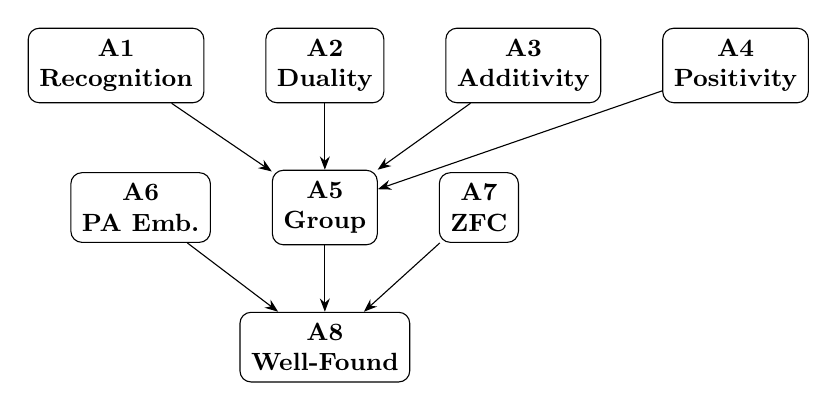
\begin{tikzpicture}[>=Stealth, node distance=22pt]
\tikzset{
  ax/.style = {draw, rectangle, rounded corners, inner sep=4pt,
               align=center, font=\small\bfseries} }
\node[ax] (A1){A1\\Recognition};
\node[ax, right=of A1] (A2){A2\\Duality};
\node[ax, right=of A2] (A3){A3\\Additivity};
\node[ax, right=of A3] (A4){A4\\Positivity};
\node[ax, below=of A2, yshift=-2pt] (A5){A5\\Group};
\node[ax, left=of A5] (A6){A6\\PA Emb.};
\node[ax, right=of A5] (A7){A7\\ZFC};
\node[ax, below=of A5, yshift=-2pt] (A8){A8\\Well-Found};

\draw[->] (A1) -- (A5);  \draw[->] (A2) -- (A5);
\draw[->] (A3) -- (A5);  \draw[->] (A4) -- (A5);
\draw[->] (A5) -- (A8);  \draw[->] (A6) -- (A8);
\draw[->] (A7) -- (A8);
\end{tikzpicture}
\end{center}

Axioms~A1--A4 feed into the algebraic structure (A5); arithmetic (A6) and
set theory (A7) backstop consistency, while A8 seals termination of proofs.
\emph{Every downstream theorem or truth-packet must cite exactly which axioms
it imports}; machine verification prohibits silent dependencies.

\section{Lean 4 Skeleton (Reference)}

For transparency, Appendix~A lists a minimal Lean~4 file that declares the
above axioms.  Future packets \texttt{import} this module and nothing else.

\section{Change-Control Policy}

\begin{itemize}
\item This document is hashed (\texttt{SHA-256} printed on the Ledger) and
  placed in the \textbf{Immutable Axiom Store}.  
\item Any proposed addition or removal requires:\par
  (i) unanimous maintainer approval, \quad
  (ii) a higher-level packet that demonstrates necessity, and\par
  (iii) a new versioned hash; old versions remain addressable.
\end{itemize}

\section*{Acknowledgments}
Thanks to the Recognition Physics Institute verification group for early
audits of the Lean formalization.

\appendix
\section{Lean 4 Stub}
\begin{verbatim}
-- genesis_axioms.lean
constant U   : Type
constant R   : U → U → Prop
constant J   : U → ℝ
constant e   : U
constant mul : U → U → U
infixl:70 " ◦ " => mul

axiom A1 : ∀ x : U, R x x
axiom A2 : ∀ x y : U, R x y ↔ R (dual y) (dual x)
axiom A3 : ∀ x y, R x y → J (x ◦ y) = J x + J y
axiom A4 : ∀ x, J x = 0 ↔ x = e
axiom A5 : (∀ x, x ◦ e = x) ∧ (∀ x, e ◦ x = x) ∧
           (∀ x, ∃ y, x ◦ y = e ∧ y ◦ x = e) ∧
           (∀ x y z, (x ◦ y) ◦ z = x ◦ (y ◦ z))
constant ℕembed : ℕ → U
axiom A6 : ∀ m n, ℕembed (m + n) = ℕembed m ◦ ℕembed n
-- A7 and A8 formalized via `universes` and `wellFounded` as needed.
\end{verbatim}

\end{document}
